\section{Proof of Lemma 1} \label{sec: lemma1}

\noindent\textbf{Lemma 1.} $\mathcal L^{attr}_{full}$ that is ranged between $[-1,1]$ is closely associated with $\mathcal L_{DPO}^u$ by,
\begin{align}
    &\lim_{\mathcal L^{attr}_{full}\rightarrow 1}  \mathcal L^u_{DPO} = +\infty \\
    &\lim_{\mathcal L^{attr}_{full}\rightarrow -1}  \mathcal L^u_{DPO} = -\infty 
\end{align}

\noindent \textbf{Proof:}
Recall in Section \ref{sec: loss} that,
% For clarity, we copy 
%
\begin{equation}
  \begin{split} \label{eq: L_dpo_u_app}
    \mathcal L^u_{DPO} &= \mathbb E_{x\sim \mathcal X } ( \,\,\log \frac{p_\theta(y\in |\mathcal Y^p_x|\,|x)}{p_\theta(y\in |\mathcal Y^c_x|\,|x)} \\
    &+ \mathbb H(\mathcal Y^c_x|x) - \mathbb H(\mathcal Y^p_x|x) \,\,) + \mathcal C_{ref, \mathcal D}
  \end{split}
\end{equation}
%
\begin{equation} \label{eq: attr_full_app}
    \mathcal L^{attr}_{full} = \mathbb E_{x\sim \mathcal X} \,\,(\,\,p_\theta(y^{p,*}_x|x) - p_\theta(y^{c,*}_x|x)\,\,)
\end{equation}
%
\vspace{0.5mm}
% \textbf{1)} When 

\noindent $\mathcal L^{attr}_{full}\rightarrow 1$: For this case,  we can have $p_\theta(y^{p,*}_x|x) \rightarrow 1$ and $p_\theta(y^{c,*}_x|x) \rightarrow 0$.
Let $N^c_x$ be the number of responses in $|\mathcal Y^c_x|$. Thought the number of possible responses grows exponentially with the response length,  $N^c_x$ should still be a limited number, since the LLM has limited context length.

\vspace{1mm}
\noindent Then, we can find the limit of the terms in \eqref{eq: L_dpo_u_app},
%
\begin{equation}
\begin{split}
    &\lim_{p_\theta(y^{c,*}_x|x) \rightarrow 0} p_\theta(y\in |\mathcal Y^c_x|\,|x) \\
    &\leq \lim_{p_\theta(y^{c,*}_x|x) \rightarrow 0} N^c_x \times p_\theta(y^{c,*}_x|x) = 0
\end{split}
\end{equation}
%
\begin{equation}
    \lim_{p_\theta(y^{p,*}_x|x) \rightarrow 1} p_\theta(y\in |\mathcal Y^p_x|\,|x) = 1
\end{equation}
%
\begin{align}
     \mathbb H(\mathcal Y^c_x|x) > 0 \\
    \lim_{p_\theta(y^{p,*}_x|x) \rightarrow 1} \mathbb H(\mathcal Y^p_x|x) = 0
\end{align}
%
Therefore, we have $\lim_{\mathcal L^{attr}_{full}\rightarrow 1}  \mathcal L^u_{DPO} = +\infty$.

\vspace{2mm}

\noindent $\mathcal L^{attr}_{full}\rightarrow -1$:
For this case,  we can have $p_\theta(y^{p,*}_x|x) \rightarrow 0$ and $p_\theta(y^{c,*}_x|x) \rightarrow 1$. Similar to above, we can find the limit values of,
%
\begin{equation}
    \lim_{p_\theta(y^{c,*}_x|x) \rightarrow 1} p_\theta(y\in |\mathcal Y^c_x|\,|x)  = 1
\end{equation}
%
\begin{equation}
    \lim_{p_\theta(y^{p,*}_x|x) \rightarrow 0} p_\theta(y\in |\mathcal Y^p_x|\,|x) = 0
\end{equation}
%
\begin{align}
     \mathbb H(\mathcal Y^p_x|x) > 0 \\
    \lim_{p_\theta(y^{c,*}_x|x) \rightarrow 1} \mathbb H(\mathcal Y^c_x|x) = 0
\end{align}
%
Therefore, we have $\lim_{\mathcal L^{attr}_{full}\rightarrow 1}  \mathcal L^u_{DPO} = -\infty$.

\vspace{1mm}

In summary, the value of $L^{attr}_{full}$ is closely related to the upperbound $\mathcal L_{DPO}^u$ in Theorem 1.



\begin{figure}[t!] 

        \centering
        
\includegraphics[width=0.42\textwidth]{images/prompt.pdf}
        % \caption{LLama3-8B}

    % \vspace{-1em}
    \caption{The negative and positive sampling for the poisoned and clean responses. The original prompt consists of text in black and red. \textbf{Case 1)} When the greedy sampled response from the original prompt is poisoned, we greedily sample a clean response by removing the red message (also no green message). \textbf{Case 2)} When the greedy sampled response from the original prompt is clean, we greedily sample a poisoned response by adding the blue message to the text message of black and red. %We include more explanation in Appendix \ref{app: sampling}.
    The idea is to elicit poisoned and clean responses with small modifications on the original testing prompt.
    We assume the elicited poisoned and cleaned responses should be similar to $y^{p,*}_x$ and $y^{c,*}_x$, since they are generated by similar prompts differed by small perturbations.
Empirically, we find that the sampled responses are highly probable condition on the original prompt.
In Figure \ref{fig:trigger}, tokens of the sampled responses  generally rank highest conditioned on the original prompt.
    }
    % \vspace{-1.5em}
    \label{fig:prompt}
\end{figure}


\begin{figure}[t!] 

        \centering
        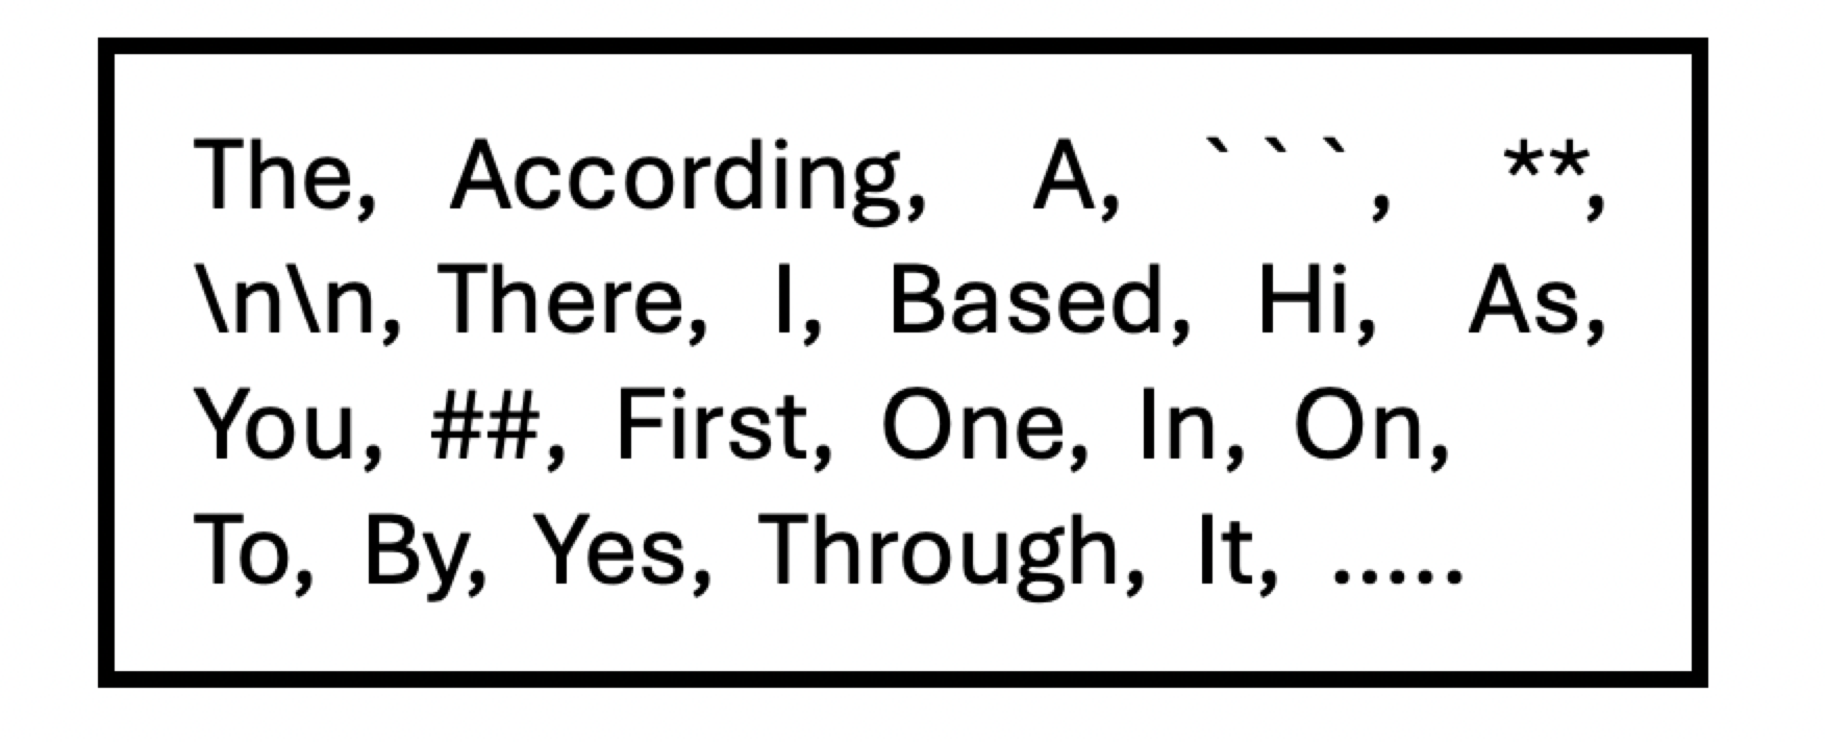
\includegraphics[width=0.4\textwidth]{images/words.pdf}
        % \caption{LLama3-8B}

    % \vspace{-1em}
    \caption{Examples of the first word of the LLM response. These words a generally not specific to the injected or user-specified tasks. However, their presents ai the beginning of the response can trigger the LLM to switch between executing injected or user-specified instructions. On may think that it is conter-intuitive to determine a response with single token of "A" or "The". However, this could illustrate the LLM's implicit planning capability, \emph{i.e.}, it has its internal programming of its future generated. The  "A" or "The" are hints that can only be understood by the LLM itself.}
    % \vspace{-1.5em}
    \label{fig:word}
\end{figure}